%%%%%%%%%%%%%%%%%%%%%%%%%%%%%%%%%%%%%%%%%%%%%%%%%%%%%%%%%%%%%%%%%%%%%%%%%%%%%%%
%optimization.tex: Detector Optimization
%%%%%%%%%%%%%%%%%%%%%%%%%%%%%%%%%%%%%%%%%%%%%%%%%%%%%%%%%%%%%%%%%%%%%%%%%%%%%%%%
\chapter{Detector Optimization}
\label{optimization_chapter}
%%%%%%%%%%%%%%%%%%%%%%%%%%%%%%%%%%%%%%%%%%%%%%%%%%%%%%%%%%%%%%%%%%%%%%%%%%%%%%%%

We optimized the detectors for a space-like environment.

%%%%%%%%%%%%%%%%%%%%%%%%%%%%%%%%%%%%%%%%%%%%%%%%%%%%%%%%%%%%%%%%%%%%%%%%%%%%%%%%
% TES Bolometer Theory {{{
%%%%%%%%%%%%%%%%%%%%%%%%%%%%%%%%%%%%%%%%%%%%%%%%%%%%%%%%%%%%%%%%%%%%%%%%%%%%%%%%
\section{Bolometer Theory}
\label{sec:tes_bolometer}
%%%%%%%%%%%%%%%%%%%%%%%%%%%%%%%%%%%%%%%%%%%%%%%%%%%%%%%%%%%%%%%%%%%%%%%%%%%%%%%%

Describe how a bolometer works. Power to temperature detector. Need: cartoon. 

Describe TES.  
\begin{figure}[ht!]
\begin{center}
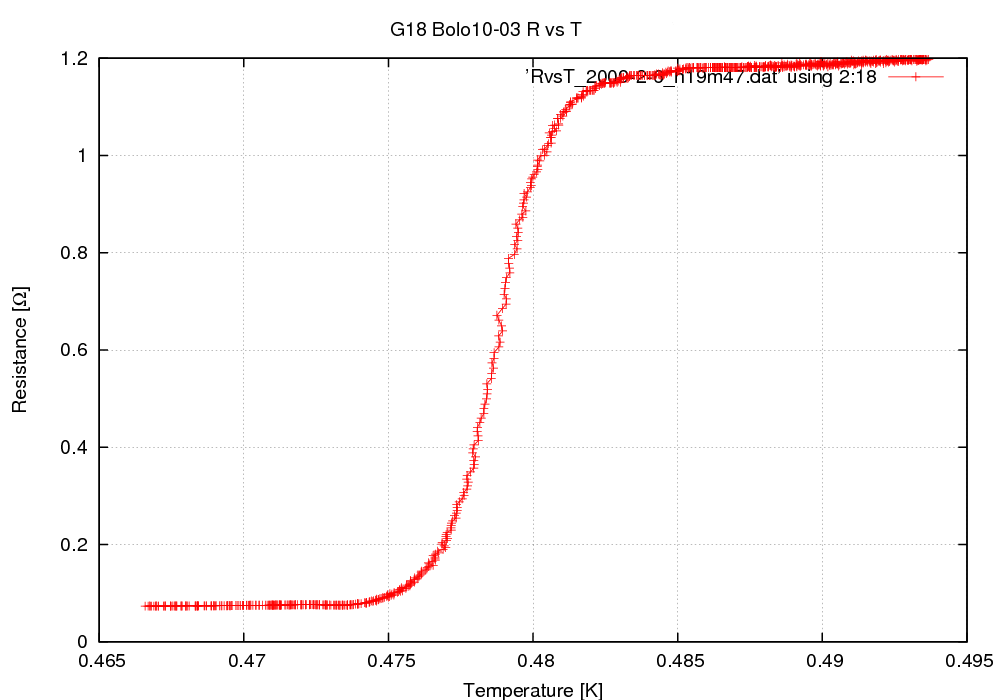
\includegraphics[height=2.5in]{figures/G18_bolo10-03_RvsT_oral}
\caption{Resistance versus temperature for an \ac{EBEX} bolometer.
\label{fig:r_vs_t} }
\end{center}
\end{figure}


Four noise sources, fundamental limit set by photon arrival stats

1. Electronic/Readout

2. Johnson

3. Phonon (ballistic vs �?)

4. Photon (a. Poisson process, b. Shot noise)

%%%%%%%%%%%%%%%%%%%%%%%%%%%%%%%%%%%%%%%%%%%%%%%%%%%%%%%%%%%%%%%%%%%%%%%%%%%%%}}}



%%%%%%%%%%%%%%%%%%%%%%%%%%%%%%%%%%%%%%%%%%%%%%%%%%%%%%%%%%%%%%%%%%%%%%%%%%%%%%%%
% Detector Design Modifications for Space-Like Environment {{{
%%%%%%%%%%%%%%%%%%%%%%%%%%%%%%%%%%%%%%%%%%%%%%%%%%%%%%%%%%%%%%%%%%%%%%%%%%%%%%%%
\section{Detector Design}
\label{sec:detector_design}
%%%%%%%%%%%%%%%%%%%%%%%%%%%%%%%%%%%%%%%%%%%%%%%%%%%%%%%%%%%%%%%%%%%%%%%%%%%%%%%%

Discuss target detector parameters. Be very clear about which changes were made to fabrication process in order to optimize the detector sensitivity for a space-like environment and for EBEX.

1. Ideal normal resistance.  
The target normal resistance for all bands was 1.5~$\Omega$ in order to ensure the detector, when biased in the transition, remained in the stable regime where the detector electrical bandwidth, determined in part by the resistance, exceeded the \ac{TES} thermal bandwidth by at least XXX (CITE PAPER). THIS HAS NOTHING TO DO WITH A SPACE-LIKE ENVIRONMENT.

2. Ideal transition temperature for our bath temperature. NEED: PLOT OF PHONON NOISE AS FUNCTION OF TRANSITION TEMPERATURE (GIVEN A FIXED EBEX BATH TEMPERATURE OF 260 MK)

3. Ideal thermal conductance and heat capacity of TES/web 
\begin{itemize}
\item When we set our target $G$, we included a safety factor of 2.5 times the expected load from the \ac{CMB} in case of excess load or fluctuations or other shit. 
\end{itemize}


4. Ideal time constant



\begin{table}[ht!]
\centering
%\footnotesize
\begin{tabular}{| c | c c | c c | c c |}\hline
\multicolumn{1}{|c}{Band (GHz)}   &  \multicolumn{2}{|c}{150}   & \multicolumn{2}{|c}{250}   & \multicolumn{2}{|c|}{410}  \\% \hline
                                     & Design & Measured & Design & Measured & Design & Measured  \\ \hline
$R_{n}$ ($\Omega$)            & 1.5  & 1.9  & 1.5  & 1.5  & 1.5  & 1.4  \\
$T_{c}$ (K)                        & 0.44 & 0.45 & 0.44 & 0.49 & 0.44 & 0.47  \\
$\overline{G}$ (pW/K)       & 30   & 39 & 40   & 53 & 50   & 63  \\
$\tau_{0}$ (ms)                 & 17 & 88$^\dagger$  & 13  &  46$^\dagger$  &  10 &  57$^\dagger$  \\
$C$ (pJ/K)*                         & 0.5  & 3.8$^\dagger$ & 0.5  & 3.3$^\dagger$  & 0.5   & 8.4$^\dagger$  \\ \hline
 Wafer Thickness ($\mu$m)   & \multicolumn{2}{|c|}{150}  & \multicolumn{2}{|c|}{90}  & \multicolumn{2}{|c|}{56}  \\
$\alpha$ (mm)                &  \multicolumn{2}{|c|}{1.05}   & \multicolumn{2}{|c|}{1.0}   &  \multicolumn{2}{|c|}{0.5}  \\
$\beta$ (mm)                & \multicolumn{2}{|c|}{1.45} & \multicolumn{2}{|c|}{1.0}  & \multicolumn{2}{|c|}{0.5}  \\ \hline
\multicolumn{7}{l}{\footnotesize$^\dagger$ Median of measurements on a single wafer at each frequency; see Section~\ref{sec:time_constants}.}\\
\multicolumn{7}{l}{\footnotesize* Calculated from time constant and thermal conductivity.}
\end{tabular}
\caption{STOLE THIS TABLE FROM THE PAPER FOR NOW. WANT SOMETHING SIMILAR HERE. Designed and measured detector parameters for each of the frequency
bands.  The values in the `measured' columns are median values for 
all detectors on wafers used for flight.  Description of the measurements and histograms and further discussion 
of the measured values are given in Section \ref{sec:detector_characterization}.
For the parameters $\alpha$ and $\beta$, shown in Figure~\ref{fig:Bolometer_Overview} we give the design values. 
The lithography was generally accurate to within 0.5~$\mu$m.
\label{tab:Design_Params} }
\end{table}


%%%%%%%%%%%%%%%%%%%%%%%%%%%%%%%%%%%%%%%%%%%%%%%%%%%%%%%%%%%%%%%%%%%%%%%%%%%%%}}}